\documentclass[a4paper,12pt]{article}
\usepackage[top = 2.5cm, bottom = 2.5cm, left = 2.5cm, right = 2.5cm]{geometry}
% Unfortunately, LaTeX has a hard time interpreting German Umlaute. The following two lines and packages should help. If it doesn't work for you please let me know.
\usepackage[T1]{fontenc}
\usepackage[utf8]{inputenc}
% The following two packages - multirow and booktabs - are needed to create nice looking tables.
\usepackage{multirow} % Multirow is for tables with multiple rows within one cell.
\usepackage{booktabs} % For even nicer tables.
% As we usually want to include some plots (.pdf files) we need a package for that.
\usepackage{graphicx}
\usepackage{tikz}
% The default setting of LaTeX is to indent new paragraphs. This is useful for articles. But not really nice for homework problem sets. The following command sets the indent to 0.
\usepackage[spanish]{babel}
\usepackage{setspace}
\setlength{\parindent}{0in}
% Package to place figures where you want them.
\usepackage{float}
% The fancyhdr package let's us create nice headers.
\usepackage{fancyhdr}
\usepackage{amsmath}
\usepackage{amssymb}
\usepackage{natbib}
\usepackage{apalike}
\usepackage{graphicx}
\usepackage{subcaption}
\usepackage{booktabs}
\usepackage{etoolbox}
\usepackage{amsthm}
\AtBeginEnvironment{align}{\setcounter{equation}{0}}
\newenvironment{solution}
  {\renewcommand\qedsymbol{$\blacksquare$}\begin{proof}[Solución]}
  {\end{proof}}
\pagestyle{fancy}

\fancyhf{}

\lhead{\footnotesize Parcial 2}
\rhead{\footnotesize  Rompich}
\cfoot{\footnotesize \thepage}



\begin{document}
    \thispagestyle{empty} % This command disables the header on the first page.

    \begin{tabular}{p{15.5cm}} % This is a simple tabular environment to align your text nicely
    \begin{tabbing}
    Universidad del Valle de Guatemala 
    \\
    Departamento de Matemática\\ Licenciatura en Matemática Aplicada \\ Fecha de entrega: 21 de marzo de 2021  \\
    Rudik R. Rompich   - Carné: 19857\\
    \end{tabbing}
    Estadística Matemática - Paulo Mejía \\
    \hline % \hline produces horizontal lines.
    \\
    \end{tabular} % Our tabular environment ends here.
    \vspace*{0.3cm} % Now we want to add some vertical space in between the line and our title.
    \begin{center} % Everything within the center environment is centered.
    {\Large \bf Parcial 2 
} % <---- Don't forget to put in the right number
        \vspace{2mm}
    \end{center}
    \vspace{0.4cm}


Instrucciones: Resuelva los siguientes problema. Favor hacer la solución en latex y cargar el archivo latex y pdf en la tarea de Canvas.\newline\newline 
Para la resolución de este parcial, se usarán las definiciones y teoremas de \cite{wackerly2014mathematical}.


\section{Problema 1} Sean $Y_1$ y $Y_2$ variables aleatorias continuas que tiene una función densidad conjunta:
$$
f\left(y_{1}, y_{2}\right)=\left\{\begin{array}{ll}
e^{-\left(y_{1}+y_{2}\right)} & , \quad 0 \leq y_{1}, 0 \leq y_{2} \\
0 & , \quad \text { en cualquier otro caso }
\end{array}\right.
$$
\begin{enumerate}
    \item a) Encontrar la función densidad de $U=Y_{1}+Y_{2}$.
    \begin{solution}
    Debido al método usado para el desarrollo del problema, primero se realizó el inciso \textbf{2. b)}. Simplemente consiste en derivar la función encontrada es decir: 
    \begin{align}
        f_U(u)&=\frac{dF_U(u)}{du}\\
              &= \begin{cases}ue^{-u}\qquad u\geq 0\\ 0 \qquad u<0\end{cases}
    \end{align}
    \end{solution}
    \item b) Calcular la función de distribución acumulada de $U$.
    \begin{solution}
    Para el desarrollo del problema se plantea el método de las funciones de distribución: \begin{center}
        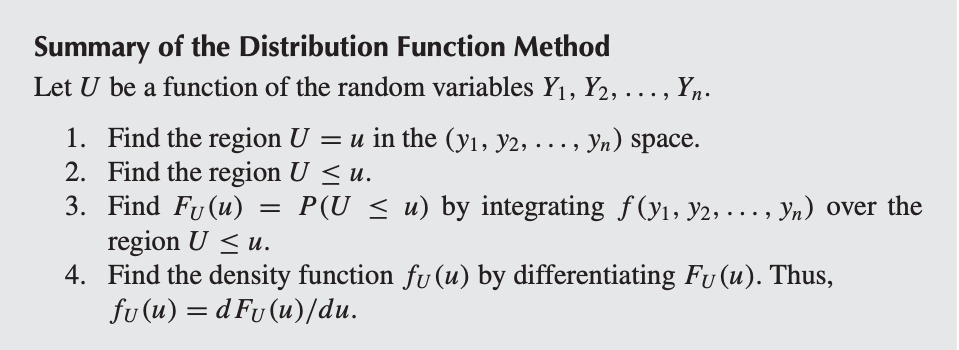
\includegraphics[scale=0.3]{images/primero.png}
    \end{center}
    Primero, se encuentra la región $U=u$, es decir, tenemos $y_1+y_2=u$: 
    \begin{center}
        

\tikzset{every picture/.style={line width=0.75pt}} %set default line width to 0.75pt        

\begin{tikzpicture}[x=0.75pt,y=0.75pt,yscale=-1,xscale=1]
%uncomment if require: \path (0,300); %set diagram left start at 0, and has height of 300

%Shape: Right Triangle [id:dp8605893718724767] 
\draw  [fill={rgb, 255:red, 208; green, 2; blue, 27 }  ,fill opacity=0.37 ][dash pattern={on 0.84pt off 2.51pt}] (231.64,78.34) -- (327.07,179.91) -- (231.64,179.91) -- cycle ;
%Shape: Axis 2D [id:dp7289302124537322] 
\draw  (218,179.91) -- (354.43,179.91)(231.64,48) -- (231.64,194.57) (347.43,174.91) -- (354.43,179.91) -- (347.43,184.91) (226.64,55) -- (231.64,48) -- (236.64,55)  ;
%Straight Lines [id:da26632778463696494] 
\draw [color={rgb, 255:red, 0; green, 0; blue, 0 }  ,draw opacity=1 ]   (231.64,78.34) -- (327.07,179.91) ;
\draw [shift={(327.07,179.91)}, rotate = 46.79] [color={rgb, 255:red, 0; green, 0; blue, 0 }  ,draw opacity=1 ][fill={rgb, 255:red, 0; green, 0; blue, 0 }  ,fill opacity=1 ][line width=0.75]      (0, 0) circle [x radius= 3.35, y radius= 3.35]   ;
\draw [shift={(231.64,78.34)}, rotate = 46.79] [color={rgb, 255:red, 0; green, 0; blue, 0 }  ,draw opacity=1 ][fill={rgb, 255:red, 0; green, 0; blue, 0 }  ,fill opacity=1 ][line width=0.75]      (0, 0) circle [x radius= 3.35, y radius= 3.35]   ;

% Text Node
\draw (358,183.21) node [anchor=north west][inner sep=0.75pt]    {$y_{1}$};
% Text Node
\draw (225,23.21) node [anchor=north west][inner sep=0.75pt]    {$y_{2}$};
% Text Node
\draw (264,56.21) node [anchor=north west][inner sep=0.75pt]    {$y_{1} +y_{2} =u\ $};
% Text Node
\draw (198,74.21) node [anchor=north west][inner sep=0.75pt]  [font=\tiny]  {$( 0,\ u)$};
% Text Node
\draw (318,187.21) node [anchor=north west][inner sep=0.75pt]  [font=\tiny]  {$( u,0)$};
% Text Node
\draw (291,114.21) node [anchor=north west][inner sep=0.75pt]    {$u\geq 0$};


\end{tikzpicture}
    \end{center}
Segundo, encontramos la región en donde $U\leq u$. Por la figura, notamos que la región es la parte inferior a la recta $u$. Si $u<0$, entonces $F_U(u)=0$. Por otra parte, si $u\geq 0$, tenemos la región en rojo.\newline\newline 

Procedemos a encontrar la región la región en rojo delimitado por $(0,0),(0,u),(u,0)$, es decir que tenemos: 
\begin{align}
F_{U}(u) &=\int_{0}^{u} \int_{0}^{-y_{1}+u} f\left(y_{1}, y_{2}\right) d y_{2} d y_{1} \\&=\int_{0}^{u} \int_{0}^{-y_{1}+u} e^{-\left(y_{1}+y_{2}\right)} d y_{2} d y_{1} \\
&=-ue^{-u}-e^{-u}+1
\intertext{Es decir, que la función de distribución acumulada es:}
F_U(u)&= \begin{cases}-ue^{-u}-e^{-u}+1\qquad u\geq 0\\ 0 \qquad u<0\end{cases}
\end{align}

    \end{solution}
    \item c) Determine el valor $E(U)$. 
    \begin{solution}
    \begin{align}
\begin{aligned}
E(U) &=\int_{-\infty}^{\infty} u f_{U}(u) d u \\
&=\int_{0}^{\infty} u\left(u e^{-u}\right) d u\\
&=\int_{0}^{\infty} u^{2} e^{-u} d u \\
&=-u^{2} e^{-u}-2 u e^{-u}-\left.2 e^{-u}\right|_{0} ^{\infty}\\
&=2
\end{aligned}
\end{align}
    \end{solution}
\end{enumerate}



(Valor 25 puntos).
%---------------------
\section{Problema 2} 
Sean $Y_{1}$ y $Y_{2}$ variables aleatorias de Poisson independientes con medias $\lambda_{1} $ y $\lambda_{2}$
\begin{enumerate}
  \item a) Encontrar la función generadora de momentos de la variable aleatoria $Y_{1}$.
  \begin{solution}
  En el Apéndice 2 - Cuadro 1, se ofrece la función generadora de momentos para Poisson.
  \begin{center}
      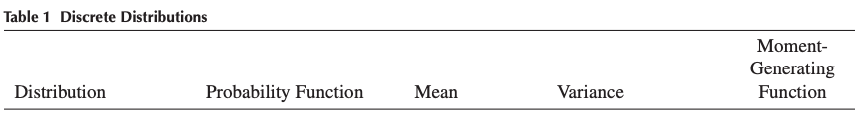
\includegraphics[scale=0.5]{images/header.png}
  \end{center}
  \begin{center}
      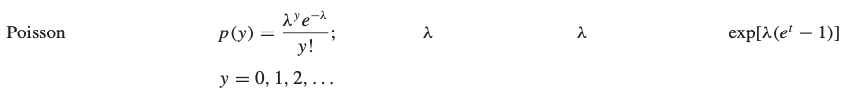
\includegraphics[scale=0.5]{images/poisson.png}
  \end{center}
  La deducción para \textit{el caso general} es la siguiente:
  \begin{align}
     m_U(t) &=E(e^{tU}) & \\
            &= \sum_{U=0}^\infty e^{tU}\cdot p(U) &\text{Definición 5.9}\\
            &= \sum_{U=0}^\infty e^{tU}\cdot \frac{\lambda^Ue^{-\lambda}}{U!} & U=0,1,2,...\\
            &= e^{-\lambda}\sum_{U=0}^\infty \frac{e^{tU}\lambda^U}{U!} =  e^{-\lambda}\sum_{U=0}^\infty \frac{(e^{t}\lambda)^U}{U!}  & 
            \intertext{Se observa que se tiene una serie de una función exponencial, i.e. $\sum_{k=0}^{\infty}\frac{z^k}{k!}=e^z$. }
            &= e^{-\lambda}e^{e^t\lambda} = e^{-\lambda +e^t\lambda}= e^{\lambda(e^t-1)}
            \intertext{Expresando la solución en una notación más clara:}
            &= \exp[\lambda(e^t-1)]
            \intertext{Entonces, para el caso específico de $Y_1$, se tiene:}
            m_{Y_1}(t) &= \exp[\lambda_1(e^{t}-1)]
            \intertext{Analogámente para $Y_2$: }
            m_{Y_2}(t) &= \exp[\lambda_2(e^{t}-1)]
  \end{align}
  \end{solution}
  \item b) Determinar la función generadora de momentos de la variable aleatoria $Y_{1}+Y_{2}$.
  \begin{solution}
  Tomando como referencia el Teorema 6.2: 
  \begin{center}
      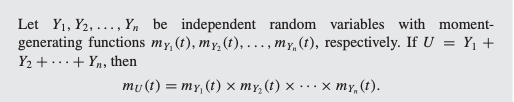
\includegraphics[scale=0.5]{images/theo6_2.png}
\begin{align}
m_{Y_1+Y_2} &= m_{Y_1}(t)\times m_{Y_2}(t) & \\
            &= \exp[\lambda_1(e^{t}-1)] \times \exp[\lambda_2(e^{t}-1)]\\
            &= \exp[\lambda_1(e^{t}-1)+\lambda_2(e^{t}-1)]
            \intertext{Entonces, tenemos la función generadora de momentos $(Y_1+Y_2)$ con media $\lambda_1+\lambda_2$:}
            &= \exp[(\lambda_1+\lambda_2)(e^{t}-1)]
\end{align}
  \end{center}
  \end{solution}
  \item c) Encontrar la función de probabilidad de $Y_{1}+Y_{2},$ utilizando los incisos b) $\mathrm{y}$ a).
  \begin{solution}
  Es decir, usando nuevamente el Cuadro 1 - Apéndice 2, se necesita regresar la función generadora de momentos a su expresión original: 
  $$m_{Y_1+Y_2}=\exp[(\lambda_1+\lambda_2)(e^{t}-1)]$$
  Es decir, que tenemos:
  $$P(Y_1+Y_2)= \frac{(\lambda_1+\lambda_2)^{Y_1+Y_2}e^{-(\lambda_1+\lambda_2)}}{(Y_1+Y_2)!}$$
  \end{solution}
  \item d) Determinar la función de probabilidad condicional de $Y_{1},$ dado $Y_{1}+Y_{2}=m$. 
  \begin{solution}
  Como es ampliamente conocido, la probabilidad condicional de una variable A dado una variable B , se calcula con $P(A|B) = \frac{P(A\cap B)}{P(B)}$. Además, como sabemos que el problema trata con variables independientes, entonces la ecuación queda como: $P(A|B) = \frac{P(A)P(B)}{P(B)}$. Usaremos la notación usual, $Y_n$ es la variable aleatoria y $y_n$ es un valor particular de $Y_n$. Entonces: 
  \begin{align}
      P(Y_1=y_1| Y_1+Y_2=m) &= \frac{P(Y_1=y_1)P(Y_1+Y_2=m)}{P(Y_1+Y_2=m)}
      \intertext{Como tenemos que encontrar la probabilidad condicional de $Y_1$ dado $Y_1+Y_2=m$ y desconocemos la probabilidad de $Y_2$, por lo que es necesario despejar $Y_2$: }
    &= \frac{P(Y_1=y_1)P(Y_2=m-y_1)}{P(Y_1+Y_2=m)}
    \intertext{Considerando la función probabilidad de Poisson:}
    &= \frac{\frac{\lambda_{1}^{y_{1}} e^{-\lambda_{1}}}{y_{1} !}\left(\frac{\lambda_{2}^{m-y_{1}} e^{-\lambda_{2}}}{\left(m-y_{1}\right) !}\right)}{\frac{\left(\lambda_{1}+\lambda_{2}\right)^{m} e^{-\left(\lambda_{1}+\lambda_{2}\right)}}{m !}}
    \intertext{Luego de hacer el desarrollo algebraico, notamos que la distribución binomial, especifícamente la función de masa de probabilidad, aparece. $P_k= \binom{n}{k}p^k(1-p)^{n-k}$, en donde $\binom{n}{k} =\frac{n!}{k!(n-k)!}$ , por lo que el resultado es:}
    &=\left(\begin{array}{c}m \\ y_{1}\end{array}\right)\left(\frac{\lambda_{1}}{\lambda_{1}+\lambda_{2}}\right)^{y_{1}}\left(1-\frac{\lambda_{1}}{\lambda_{1}+\lambda_{2}}\right)^{m-y_{1}} 
  \end{align}

  \end{solution}
\end{enumerate}
(Valor 25 puntos).
\section{Problema 3}
 Los tiempos de servicio para los clientes que pasan por una caja de un supermercado son variables aleatorias independientes con $\mu=1.5$ minutos y $\sigma^{2}=1.0$. Se quiere calcular la probabilidad de que 100 clientes puedan ser atendidos en menos de 2 horas del tiempo total del servicio.
 \begin{enumerate}
 \item a) ¿Se puede aplicar el teorema del límite central?
\begin{solution}
Considerando el teorema de límite central: 
\begin{center}
    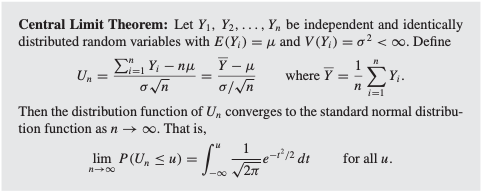
\includegraphics[scale=0.7]{images/TeoLimiteCentral.png}
\end{center}
Se sabe que si una muestra tiene más de 30 elementos, entonces se asegura que se podrá tratar aproximadamente como una distribución normal. En un contexto formal, para una distribución con un $n\to \infty$ ($n$ lo suficiente grande) entonces la probabilidad podrá ser aproximada por una distribución normal.
\newline\newline
Como nos lo asegura el teorema, ya que tenemos $\mu=1.5$, $\sigma^2=1$ y muestras $Y_1,Y_2,...,Y_{100}$. (En donde $n> 30$, que es significativo). Lo que implica que se puede definir un $U_n$. Por lo tanto, el problema cumple las condiciones adecuadas para aplicar el Teorema del Límite Central.
\end{solution}

 \item b) Calcule la probabilidad de que 100 clientes puedan ser atendidos en menos de 2 horas del tiempo total del servicio (Use $\mathrm{R}$ ).
 \begin{solution}
 Comenzamos colocando todos los datos en una misma dimensional, es decir: Media $=1.5$ minutos,  Varianza $=1$ minuto, Tiempo total de servicio $= 120$ minutos. Entonces, nos piden la probabilidad que 100 clientes puedan ser atendidos en 120 minutos, es decir, usando un \textit{script} de R: 
 \begin{center}
     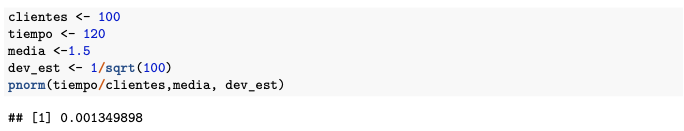
\includegraphics[scale=0.5]{images/r.png}
 \end{center}
 
 \end{solution}

 \item c) ¿Considera que es posible atender a los 100 clientes en menos de 2 horas? 
 \begin{solution}
No, ya que la probabilidad es ínfima; insignificante. Aunque puede afirmarse que no es imposible, solo que bastante improbable. 
\end{solution}
 \end{enumerate}
 (Valor 25 puntos).
\section{Problema 4} Sean $\mathrm{Y}_{1}, \mathrm{Y}_{2}, \ldots, \mathrm{Y}_{n}$ variables aleatorias normales e independientes, cada una con media $\mu$ y varianza $\sigma^{2}$.
\begin{enumerate}
\item a) Determine la distribución de $\sqrt{n}\left(\frac{\bar{Y}-\mu}{\sigma}\right)$ (no tiene que encontrar la forma cerrada de la distribución sólo indicar el tipo con sus parámetros)
\begin{solution}
Es trivial asumir que $\mu=\mu_{\bar{Y}}$ y $\sigma=\sqrt{\sigma_{\bar{Y}}^2 n}=\sigma_{\bar{Y}}\sqrt{n}$.  Entonces por el Teorema 7.1 
\begin{center}
    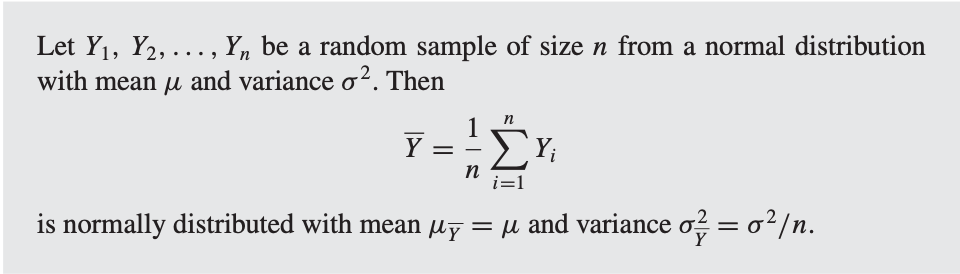
\includegraphics[scale=0.3]{images/teo7_1.png}
\end{center}
es posible asumir que tiene una distribución normal estándar. En donde: $\sigma$ = desviación estándar, $n$= número de variables, $\bar{Y}$= función de media muestral de variables aleatorias y $\mu$ = media. 
\end{solution}
\item b) Determine la distribución de $\frac{(n-1) S^{2}}{\sigma^{2}}$ (no tiene que encontrar la forma cerrada de la distribución sólo indicar el tipo con sus parámetros)
\begin{solution}
Por el Teorema 7.3 
\begin{center}
    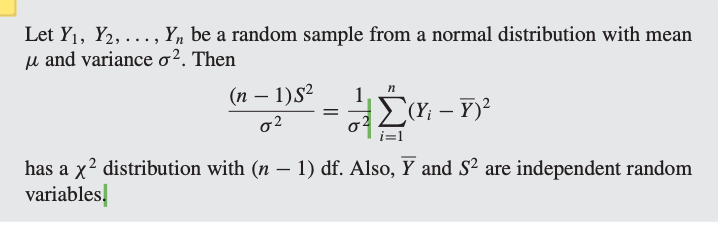
\includegraphics[scale=0.5]{images/4-2.png}
\end{center}
se puede determinar que la distribución tiene una distribución $\chi^2$ con $(n-1)$ grados de libertad. En donde: $n$ número de variables, $S^2$ varianza muestral y $\sigma^2$ la varianza.

\end{solution}
\item c) Determine la distribución de $\sqrt{n}\left(\frac{\bar{Y}-\mu}{S}\right)$ (no tiene que encontrar la forma cerrada de la distribución sólo indicar el tipo con sus parámetros)
\begin{solution}
Es un caso especial del problema \textbf{1. a)} ya que si $\sigma$ es desconocido, entonces tiene que ser estimado por $S=\sqrt{S^2}$:  Por lo que es posible asumir que tiene una distribución t de Student. En donde: $S$ = desviación estándar muestral, $n$= número de variables, $\bar{Y}$= función de media muestral de variables aleatorias y $\mu$ = media.
\end{solution}
\item d) Sean 2 muestras aleatorias independientes tomadas de distribuciones normales de tamaño $n_{1}$ y $n_{2} .$ Determine la distribución de $\frac{S_{1}^{2} / \sigma_{1}^{2}}{S_{2}^{2} / \sigma_{2}^{2}}$ (no tiene que encontrar la forma cerrada de la distribución sólo indicar el tipo con sus parámetros)
\begin{solution}
De acuerdo a la definición 7.3: 
\begin{center}
    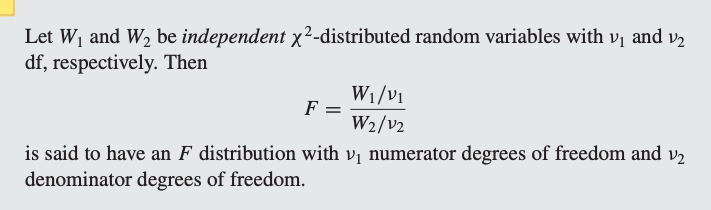
\includegraphics[scale=0.5]{images/4-d.png}
\end{center}
por la forma de la distribución, entonces esta debe tener una distribución F con $n_1-1$ grados de libertad en el numerador y $n_2-1$ en el denominador. En donde: $S_1$ y $S_2$ representan la desviación estándar muestral y $\sigma_1^2$ y $ \sigma_2^2$ representan la varianza.
\end{solution}
\end{enumerate}
(Valor 25 puntos).

\bibliographystyle{apalike}
\bibliography{bibs.bib}

\end{document}